\documentclass[11pt,aspectratio=169]{beamer}
\usepackage{amsmath,amssymb,bm,graphicx,booktabs,tikz}
\usetikzlibrary{arrows.meta}
\usetheme{default}
\setbeamertemplate{navigation symbols}{}
\setbeamertemplate{headline}{}
\setbeamertemplate{footline}{%
  \leavevmode\hbox{%
    \begin{beamercolorbox}[wd=\paperwidth,ht=2.6ex,dp=1.1ex,right]{page number in head/foot}%
      \insertframenumber/\inserttotalframenumber\hspace{0.35cm}
    \end{beamercolorbox}}}
\setbeamertemplate{frametitle}{\vspace{0.25cm}\insertframetitle\par\vspace{0.08cm}\hrule}
\setbeamercolor{normal text}{fg=black,bg=white}
\setbeamercolor{frametitle}{fg=black,bg=white}
\setbeamercolor{structure}{fg=black}
\setbeamersize{text margin left=0.7cm,text margin right=0.7cm}
\definecolor{femblue}{RGB}{47,99,143}
\definecolor{femorange}{RGB}{198,91,42}
\newcommand{\bu}{\bm u}
\newcommand{\bv}{\bm v}
\newcommand{\bw}{\bm w}
\newcommand{\bx}{\bm x}
\newcommand{\bn}{\bm n}
\newcommand{\bb}{\bm b}
\newcommand{\bt}{\bm t}
\newcommand{\bI}{\bm I}
\newcommand{\beps}{\bm\varepsilon}
\newcommand{\bsig}{\bm\sigma}
\newcommand{\Om}{\Omega}
\newcommand{\Vzero}{\mathcal V_0}
\newcommand{\Vhzero}{\mathcal V_{h,0}}
\newcommand{\dd}{\,\mathrm d}
\newcommand{\divg}{\nabla\!\cdot}
\newcommand{\norm}[2][]{\left\lVert#2\right\rVert_{#1}}
\DeclareMathOperator{\tr}{tr}
\graphicspath{{figures/}}

\begin{document}

\begin{frame}
\centering\vfill
{\LARGE\bfseries Mixed Finite Element Methods\par}
\vspace{0.45cm}
{\large Lecture 1: Near-incompressibility, locking, and pressure\par}
\vfill
\end{frame}

\begin{frame}{Lecture outline}
\begin{enumerate}
\item Relate volume change to displacement and material parameters.
\item Explain why a nearly incompressible material can be difficult to
approximate with displacement elements.
\item Examine a small mesh and a computed example of volumetric locking.
\item Introduce pressure and obtain the displacement--pressure equations.
\end{enumerate}
\vspace{0.3cm}
The model is small-strain isotropic elasticity. The two-dimensional
calculations use \textbf{plane strain}.
\end{frame}

\section{Volume change and near-incompressibility}
\begin{frame}
\centering\vfill
{\LARGE Volume change and near-incompressibility\par}
\vfill
\end{frame}

\begin{frame}{Recall: the linear-elastic problem}
The displacement is $\bu$, the strain is $\beps$, and the stress is $\bsig$:
\[
\beps(\bu)=\tfrac12(\nabla\bu+\nabla\bu^T),\qquad
\bsig(\bu)=2\mu\beps(\bu)+\lambda\tr\beps(\bu)\bI.
\]
With zero prescribed displacement, the strong problem is
\[
\left\{\begin{aligned}
-\divg\bsig(\bu)&=\rho\bb &&\text{in }\Om,\\
\bu&=\bm0 &&\text{on }\Gamma_u,\\
\bsig(\bu)\bn&=\overline{\bt} &&\text{on }\Gamma_t.
\end{aligned}\right.
\]
Here $\rho\bb$ is body force per unit volume, $\overline{\bt}$ is prescribed
traction, and $\bn$ is the outward unit normal.

Assume that the displacement boundary removes rigid motions.
\end{frame}

\begin{frame}{Displacement and volume change}
For a small material region of initial volume $V$, define the relative
volume change $\Delta V/V$. For small displacement gradients,
\[
\frac{V+\Delta V}{V}=\det(\bI+\nabla\bu)
=1+\tr(\nabla\bu)+O(\norm{\nabla\bu}^2).
\]
The \textbf{volumetric strain} is the first-order volume change:
\[
\boxed{\varepsilon_v=\frac{\Delta V}{V}\ \text{to first order}
=\tr\beps(\bu)=\divg\bu.}
\]
In three dimensions,
\[
\varepsilon_v=\frac{\partial u_1}{\partial x_1}
+\frac{\partial u_2}{\partial x_2}
+\frac{\partial u_3}{\partial x_3}.
\]
Positive $\varepsilon_v$ means expansion. Negative $\varepsilon_v$ means compression.
\end{frame}

\begin{frame}{Volume change and shape change}
Dashed outlines are undeformed. Both deformations have $u_3=0$.
\begin{columns}[T,onlytextwidth]
\begin{column}{0.48\textwidth}
\centering
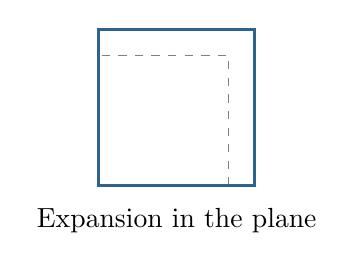
\begin{tikzpicture}[scale=1.1]
\draw[dashed,gray] (0,0) rectangle (1.5,1.5);
\draw[very thick,femblue] (0,0) rectangle (1.8,1.8);
\node[below] at (0.9,-.15) {Expansion in the plane};
\end{tikzpicture}
\[
\bu=(a x_1,a x_2,0)^T,\qquad a>0,
\]
\[
\varepsilon_v=2a,\qquad
\frac{\Delta V}{V}=2a+a^2.
\]
\end{column}
\begin{column}{0.49\textwidth}
\centering
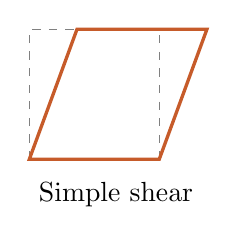
\begin{tikzpicture}[scale=1.1]
\draw[dashed,gray] (0,0) rectangle (1.5,1.5);
\draw[very thick,femorange] (0,0)--(1.5,0)--(2.05,1.5)--(.55,1.5)--cycle;
\node[below] at (1,-.15) {Simple shear};
\end{tikzpicture}
\[
\bu=(\gamma x_2,0,0)^T,
\]
\[
\varepsilon_v=0,\qquad \det(\bI+\nabla\bu)=1.
\]
\end{column}
\end{columns}
Shear changes shape while preserving volume. Incompressibility does not
require zero displacement or zero strain.
\end{frame}

\begin{frame}{Shear modulus and bulk modulus}
The shear modulus $\mu$ measures resistance to shear deformation.
Taking the trace of the three-dimensional constitutive law gives
\[
\tr\bsig=2\mu\varepsilon_v+3\lambda\varepsilon_v.
\]
Define the \textbf{bulk modulus} $\kappa$ by
\[
\boxed{\frac13\tr\bsig=\kappa\varepsilon_v,
\qquad \kappa=\lambda+\frac{2\mu}{3}.}
\]
In terms of Young's modulus $E$ and Poisson's ratio $\nu$,
\[
\mu=\frac{E}{2(1+\nu)},\qquad
\lambda=\frac{E\nu}{(1+\nu)(1-2\nu)},\qquad
\kappa=\frac{E}{3(1-2\nu)}.
\]
All four moduli have units of stress. The ratio $\kappa/\mu$ is dimensionless.
\end{frame}

\begin{frame}{Nearly incompressible material response}
As $\nu\to1/2$, the bulk modulus becomes large relative to the shear modulus:
\[
\frac{\kappa}{\mu}=\frac{2(1+\nu)}{3(1-2\nu)}.
\]
\begin{center}
\begin{tabular}{ccc}
\toprule
$\nu$ & $\lambda/\mu$ & $\kappa/\mu$\\
\midrule
0.30 & 1.5 & 2.17\\
0.49 & 49 & 49.67\\
0.4999 & 4999 & 4999.67\\
\bottomrule
\end{tabular}
\end{center}
For a bounded mean stress, $\varepsilon_v=(\tr\bsig)/(3\kappa)$ becomes small.

The material can still shear. Its resistance to volume change is much
greater than its resistance to shape change.
\end{frame}

\begin{frame}{Plane strain and plane stress are different models}
\begin{columns}[T,onlytextwidth]
\begin{column}{0.48\textwidth}
\textbf{Plane strain}
\[
\bu=(u_1(x_1,x_2),u_2(x_1,x_2),0)^T.
\]
Thus $\varepsilon_{33}=0$, but $\sigma_{33}$ can be nonzero.
\[
\varepsilon_v=\partial_1u_1+\partial_2u_2.
\]
Incompressibility requires this in-plane divergence to vanish.
\end{column}
\begin{column}{0.48\textwidth}
\textbf{Plane stress}
\[
\sigma_{33}=\sigma_{13}=\sigma_{23}=0.
\]
The thickness strain $\varepsilon_{33}$ can compensate in-plane area change.

It would be incorrect to impose
$\partial_1u_1+\partial_2u_2=0$ merely because the three-dimensional material
is incompressible.
\end{column}
\end{columns}
\vspace{0.35cm}
Our locking examples use \textbf{plane strain}, with the three-dimensional
material parameters $\lambda$ and $\mu$.
\end{frame}

\section{Volumetric locking}
\begin{frame}
\centering\vfill
{\LARGE Volumetric locking\par}
\vfill
\end{frame}

\begin{frame}{Recall: displacement variational problem}
With $\Vzero=\{\bv\in[H^1(\Om)]^d:\bv=\bm0\text{ on }\Gamma_u\}$,
define the linear functional
\[
\ell_{\mathrm{el}}(\bv)=\int_\Om\rho\bb\cdot\bv\dd x
+\int_{\Gamma_t}\overline{\bt}\cdot\bv\dd s.
\]
The displacement problem is
\[
\boxed{\text{find }\bu\in\Vzero:\quad
a_{\mathrm{el}}(\bu,\bv)=\ell_{\mathrm{el}}(\bv)
\quad\forall\bv\in\Vzero,}
\]
where
\[
a_{\mathrm{el}}(\bw,\bv)
=2\mu\int_\Om\beps(\bw):\beps(\bv)\dd x
+\lambda\int_\Om(\divg\bw)(\divg\bv)\dd x.
\]
For plane strain, $d=2$ and the out-of-plane displacement is zero.
\end{frame}

\begin{frame}{The energy cost of unintended volume change}
The finite element displacement minimizes
\[
\Pi_{\mathrm{el}}(\bu_h)
=\frac12a_{\mathrm{el}}(\bu_h,\bu_h)-\ell_{\mathrm{el}}(\bu_h)
\]
over the discrete displacement space. Expanding the elastic term,
\[
\Pi_{\mathrm{el}}(\bu_h)
=\mu\int_\Om\beps(\bu_h):\beps(\bu_h)\dd x
+\frac{\lambda}{2}\int_\Om(\divg\bu_h)^2\dd x
-\ell_{\mathrm{el}}(\bu_h).
\]
\begin{itemize}
\item A large $\lambda$ makes even a small unintended divergence expensive.
\item If the discrete space cannot represent the required deformation with
small divergence, the computed response can become artificially stiff.
\end{itemize}
This loss of approximation quality near incompressibility is
\textbf{volumetric locking}.
\end{frame}

\begin{frame}{Incompressibility on a linear triangle}
On one $P_1$ triangle, write the two displacement components as
\[
u_{h,1}=a_1+b_1x_1+c_1x_2,\qquad
u_{h,2}=a_2+b_2x_1+c_2x_2.
\]
The six coefficients determine an affine displacement field. Its divergence is
\[
\divg\bu_h
=\frac{\partial u_{h,1}}{\partial x_1}
+\frac{\partial u_{h,2}}{\partial x_2}
=b_1+c_2.
\]
Thus exact incompressibility requires $b_1+c_2=0$ throughout that triangle.

Neighboring triangles share displacement degrees of freedom. Enforcing
zero divergence on each element can severely restrict the available
deformations. We examine a small mesh to see this explicitly.
\end{frame}

\begin{frame}{A four-triangle mesh with one free node}
\begin{columns}[c,onlytextwidth]
\begin{column}{0.47\textwidth}
\centering
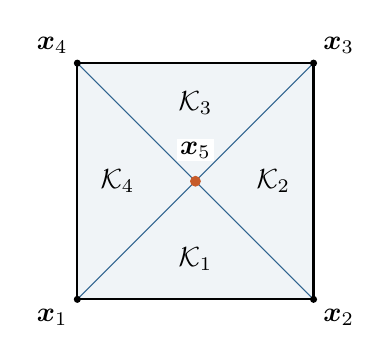
\begin{tikzpicture}[scale=3]
\fill[femblue!7] (0,0) rectangle (1,1);
\draw[thick] (0,0) rectangle (1,1);
\draw[femblue] (0,0)--(1,1) (0,1)--(1,0);
\foreach \x/\y/\lab/\pos in {0/0/1/below left,1/0/2/below right,1/1/3/above right,0/1/4/above left}{
\fill (\x,\y) circle (.015);
\node[\pos] at (\x,\y) {$\bx_{\lab}$};}
\fill[femorange] (.5,.5) circle (.023);
\node[above=7pt,fill=white,inner sep=1pt] at (.5,.5) {$\bx_5$};
\node at (.5,.17) {$\mathcal K_1$};
\node at (.83,.5) {$\mathcal K_2$};
\node at (.5,.83) {$\mathcal K_3$};
\node at (.17,.5) {$\mathcal K_4$};
\end{tikzpicture}
\end{column}
\begin{column}{0.5\textwidth}
The domain is $(0,1)^2$. All boundary displacements are zero.
\[
\bx_1=(0,0)^T,\quad\bx_2=(1,0)^T,
\]
\[
\bx_3=(1,1)^T,\quad\bx_4=(0,1)^T,
\]
\[
\bx_5=(1/2,1/2)^T.
\]
Only the center-node vector $\bm U_5=(U_{5,1},U_{5,2})^T$ is free.
\[
\bu_h=\phi_5\bm U_5.
\]
The global nodal basis function $\phi_5$ is one at the center and zero at
the corners.
\end{column}
\end{columns}
\end{frame}

\begin{frame}{Divergence of the center-node displacement}
Since $\bm U_5$ is constant,
\[
\divg\bu_h=U_{5,1}\partial_1\phi_5+U_{5,2}\partial_2\phi_5.
\]
On each triangle, the affine function that has the required nodal values gives
\begin{center}
\begin{tabular}{ccc}
\toprule
Element & $\phi_5$ restricted to the element & $\divg\bu_h$\\
\midrule
$\mathcal K_1$ & $2x_2$ & $2U_{5,2}$\\[0.15em]
$\mathcal K_2$ & $2(1-x_1)$ & $-2U_{5,1}$\\[0.15em]
$\mathcal K_3$ & $2(1-x_2)$ & $-2U_{5,2}$\\[0.15em]
$\mathcal K_4$ & $2x_1$ & $2U_{5,1}$\\
\bottomrule
\end{tabular}
\end{center}
For example, on $\mathcal K_1$, $\partial_1\phi_5=0$ and
$\partial_2\phi_5=2$, giving $\divg\bu_h=2U_{5,2}$.
\end{frame}

\begin{frame}{The constraint leaves only zero displacement on this mesh}
The incompressibility conditions on the bottom and right triangles give
\[
2U_{5,2}=0,\qquad -2U_{5,1}=0.
\]
Consequently,
\[
\boxed{\bm U_5=\bm0,\qquad \bu_h=\bm0.}
\]
On this particular mesh, the space contains no nonzero displacement that
both vanishes on the boundary and has zero divergence on every element.

For nearly incompressible material, a large $\lambda$ strongly discourages
the remaining nonzero displacement modes.

This calculation isolates the restriction imposed by the discrete space.
A computed problem will show its effect on approximation error.
\end{frame}

\begin{frame}{A computed test with a fixed exact displacement}
Use plane strain on $\Om=(0,1)^2$, with $\bu=\bm0$ on the whole boundary.
Let $a_0=10^{-3}$ and prescribe the manufactured displacement
\[
\bu_{\mathrm{ex}}=a_0
\begin{bmatrix}
\sin^2(\pi x_1)\sin(2\pi x_2)\\
-\sin(2\pi x_1)\sin^2(\pi x_2)
\end{bmatrix}.
\]
Both components vanish on the boundary. Direct differentiation gives
\[
\partial_1u_{\mathrm{ex},1}
=a_0\pi\sin(2\pi x_1)\sin(2\pi x_2)
=-\partial_2u_{\mathrm{ex},2},
\]
so $\divg\bu_{\mathrm{ex}}=0$ exactly.
\end{frame}

\begin{frame}{The load does not change as the bulk modulus increases}
For constant material parameters, the displacement equation is
\[
-\divg\bsig(\bu)
=-\mu\Delta\bu-(\lambda+\mu)\nabla(\divg\bu)=\rho\bb.
\]
Substituting $\bu=\bu_{\mathrm{ex}}$ and $\divg\bu_{\mathrm{ex}}=0$ gives
\[
\boxed{\rho\bb=-\mu\Delta\bu_{\mathrm{ex}}.}
\]
Hold $\mu=1$ and this load fixed. Vary $\nu$, setting
$\lambda=2\mu\nu/(1-2\nu)$ and $\kappa=\lambda+2\mu/3$.

The exact displacement remains unchanged. Thus a decreasing computed
response cannot be explained by physical stiffening of this exact solution.
\[
u_{\mathrm{ex},1}(1/2,1/4)=a_0\qquad\text{for every material parameter tested.}
\]
\end{frame}

\begin{frame}{Computed displacement response near incompressibility}
\centering
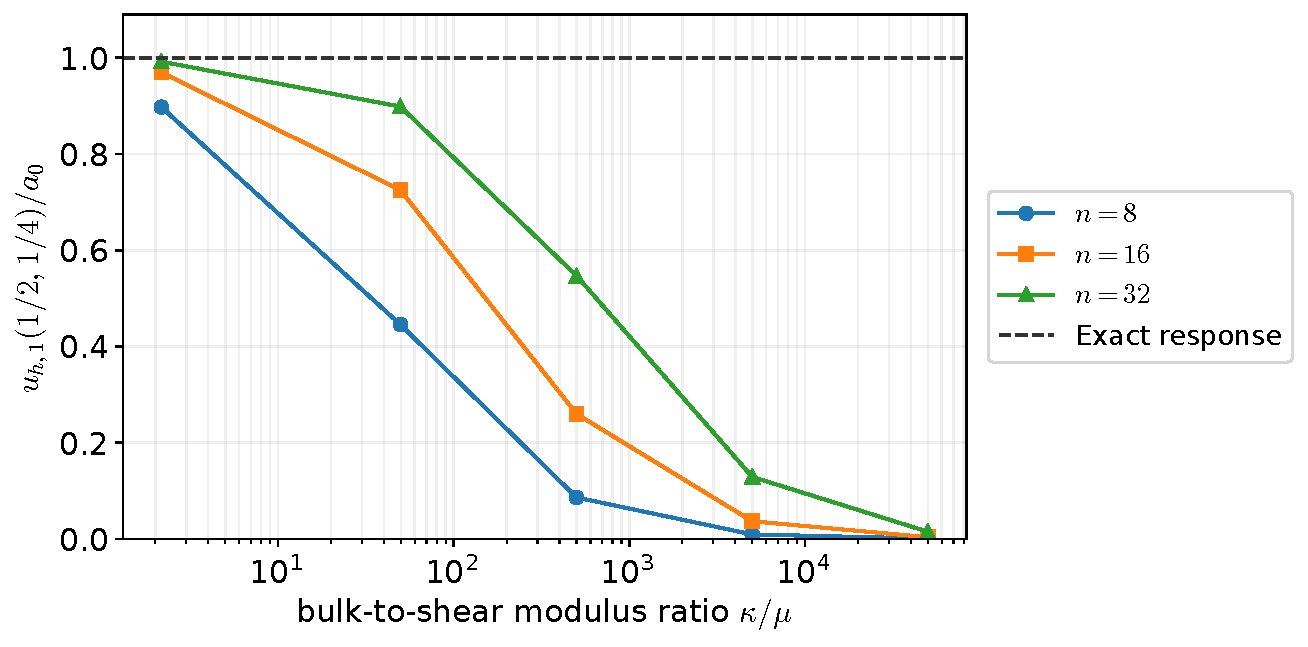
\includegraphics[width=0.92\textwidth,height=0.63\textheight,keepaspectratio]{locking_response.pdf}
\par\vspace{0.1cm}
\raggedright
Each mesh has $n\times n$ squares, split into $2n^2$ linear triangles.
The dashed line is the exact response, equal to one after normalization.
Increasing $\kappa/\mu$ suppresses the computed displacement on a fixed mesh.
\end{frame}

\begin{frame}{Refinement helps, but the material parameter matters}
\centering
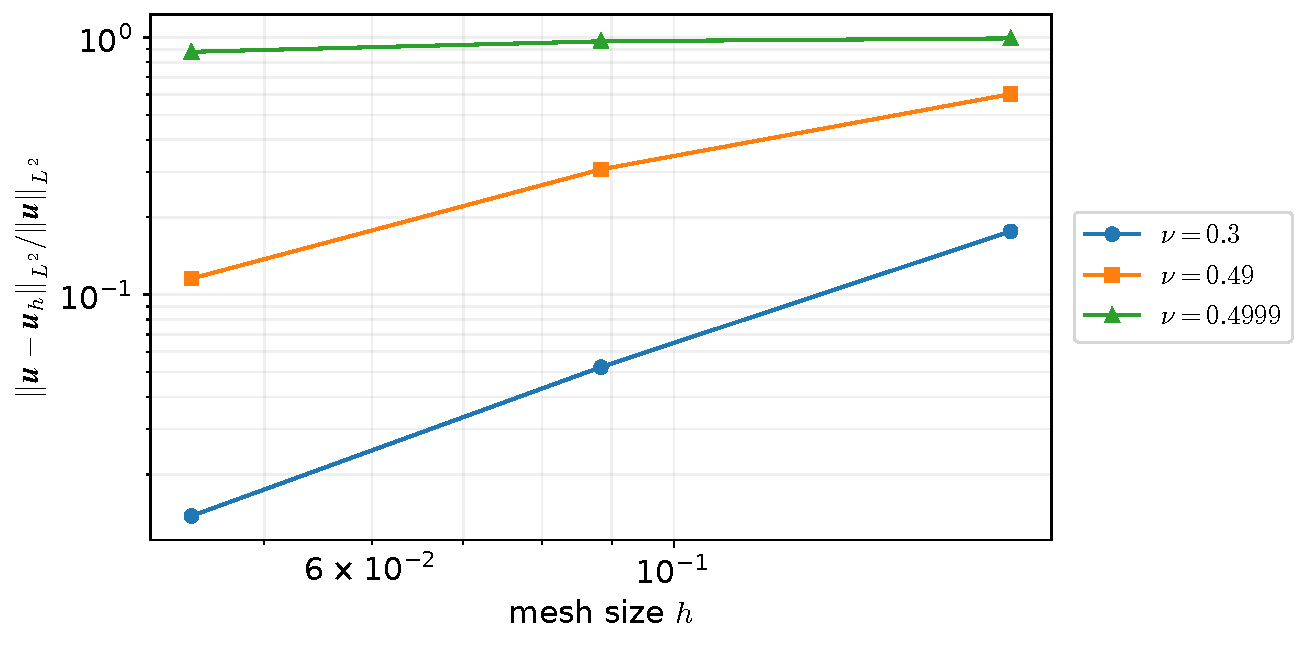
\includegraphics[width=0.92\textwidth,height=0.63\textheight,keepaspectratio]{locking_mesh_error.pdf}
\par\vspace{0.1cm}
\raggedright
The error uses the analytic displacement, not its nodal interpolant.
These are results for the displacement-only $P_1$ method on the stated meshes.
Locking does not mean that mesh refinement can never improve the solution.
\end{frame}

\begin{frame}{Connection to the error estimates in Chapter 7}
With the displacement boundary removing rigid motions, Korn's inequality gives
\[
\norm[L^2]{\beps(\bv)}^2\ge c_K\norm[H^1]{\bv}^2,
\qquad c_K>0.
\]
For $\lambda\ge0$, coercivity does not deteriorate as $\lambda$ increases:
\[
a_{\mathrm{el}}(\bv,\bv)\ge2\mu c_K\norm[H^1]{\bv}^2.
\]
But continuity in three dimensions gives the bound
\[
|a_{\mathrm{el}}(\bw,\bv)|
\le(2\mu+3\lambda)\norm[H^1]{\bw}\norm[H^1]{\bv}.
\]
Thus we may take $\alpha=2\mu c_K$ and $M=2\mu+3\lambda$.
\end{frame}

\begin{frame}{A material-dependent error bound}
Recall C\'ea's estimate in the $H^1$ norm:
\[
\norm[H^1]{\bu-\bu_h}
\le\frac{M}{\alpha}\inf_{\bv_h\in\Vhzero}\norm[H^1]{\bu-\bv_h}.
\]
Substituting the continuity and coercivity constants from the previous slide,
\[
\frac{M}{\alpha}=\frac{2\mu+3\lambda}{2\mu c_K}
\longrightarrow\infty\quad\text{as }\lambda\to\infty\text{ with }\mu\text{ fixed}.
\]
The best-approximation error may decrease as the mesh is refined, but this
$H^1$ bound does not give a constant uniform in incompressibility.

A growing upper bound alone does not prove locking. The computed errors
show the actual deterioration for the tested displacement elements.
\end{frame}

\section{Pressure as an additional unknown}
\begin{frame}
\centering\vfill
{\LARGE Pressure as an additional unknown\par}
\vfill
\end{frame}

\begin{frame}{Separating volumetric and deviatoric strain}
Define the \textbf{deviatoric strain}, the trace-free part of the strain tensor:
\[
\beps_{\mathrm{dev}}(\bu)
=\beps(\bu)-\frac{\varepsilon_v}{3}\bI,
\qquad \tr\beps_{\mathrm{dev}}=0.
\]
Substitute $\beps=\beps_{\mathrm{dev}}+(\varepsilon_v/3)\bI$ into Hooke's law:
\[
\begin{aligned}
\bsig
&=2\mu\beps_{\mathrm{dev}}+
   \left(\lambda+\frac{2\mu}{3}\right)\varepsilon_v\bI\\
&=2\mu\beps_{\mathrm{dev}}+\kappa\varepsilon_v\bI.
\end{aligned}
\]
The factor $1/3$ refers to the \textbf{three-dimensional} strain tensor.
In plane strain, retain this definition and set $\varepsilon_{33}=0$.
\end{frame}

\begin{frame}{The three-dimensional strain in a plane-strain calculation}
For $\bu=(u_1(x_1,x_2),u_2(x_1,x_2),0)^T$, the strain is
\[
\beps=
\begin{bmatrix}
\partial_1u_1 & (\partial_2u_1+\partial_1u_2)/2 & 0\\
(\partial_2u_1+\partial_1u_2)/2 & \partial_2u_2 & 0\\
0&0&0
\end{bmatrix}.
\]
Its trace is $\varepsilon_v=\partial_1u_1+\partial_2u_2$, but
\[
\varepsilon_{\mathrm{dev},33}=-\frac{\varepsilon_v}{3},
\qquad \sigma_{33}=\lambda\varepsilon_v.
\]
Thus the deviatoric strain can have a nonzero third normal component even
though $\varepsilon_{33}=0$. The pressure below is the mean of all three
normal stresses.
\end{frame}

\begin{frame}{Pressure and its sign convention}
\begin{columns}[c,onlytextwidth]
\begin{column}{0.64\textwidth}
Define pressure as minus the mean normal stress:
\[
\boxed{p=-\frac13\tr\bsig=-\kappa\varepsilon_v
=-\kappa\divg\bu.}
\]
The stress becomes
\[
\boxed{\bsig=2\mu\beps_{\mathrm{dev}}(\bu)-p\bI.}
\]
\begin{itemize}
\item Compression: $\varepsilon_v<0$, so $p>0$.
\item Hydrostatic stress: $\bsig=-p\bI$.
\end{itemize}
\end{column}
\begin{column}{0.32\textwidth}
\centering
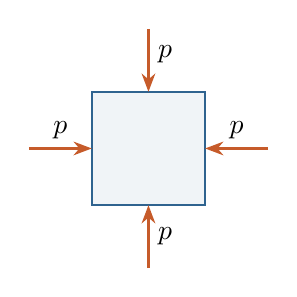
\begin{tikzpicture}[scale=.8,>=Stealth]
\fill[femblue!7] (0,0) rectangle (1.8,1.8);
\draw[thick,femblue] (0,0) rectangle (1.8,1.8);
\draw[->,thick,femorange] (-1,.9)--(0,.9);
\draw[->,thick,femorange] (2.8,.9)--(1.8,.9);
\draw[->,thick,femorange] (.9,2.8)--(.9,1.8);
\draw[->,thick,femorange] (.9,-1)--(.9,0);
\node[above] at (-.5,.9) {$p$};
\node[above] at (2.3,.9) {$p$};
\node[right] at (.9,2.4) {$p$};
\node[right] at (.9,-.5) {$p$};
\end{tikzpicture}
\[
\bsig\bn=-p\bn,\quad p>0.
\]
\end{column}
\end{columns}
\vspace{0.15cm}
For example, $\beps=-\delta\bI$ with $\delta>0$ gives
$\varepsilon_v=-3\delta$ and $p=3\kappa\delta>0$.
\end{frame}

\begin{frame}{Zero volume change does not imply zero pressure}
Consider a fixed hydrostatic pressure $p_0>0$. The constitutive relation gives
\[
\varepsilon_v=-\frac{p_0}{\kappa}.
\]
As $\kappa\to\infty$,
\[
\varepsilon_v\longrightarrow0,\qquad p=p_0\ne0.
\]
Thus we cannot first set $\divg\bu=0$ and then infer that
$p=-\kappa\divg\bu$ vanishes in the incompressible limit.

Pressure can remain finite while the volume change tends to zero.
Treating pressure as an unknown lets us retain this stress without computing
it solely as a large modulus times a small displacement divergence.
\end{frame}

\begin{frame}{The displacement--pressure strong problem}
For finite $\kappa$, replace the displacement-only constitutive equation by
\[
\bsig=2\mu\beps_{\mathrm{dev}}(\bu)-p\bI,
\qquad \divg\bu+\frac{p}{\kappa}=0.
\]
The strong problem for the two unknown fields $\bu$ and $p$ is
\[
\left\{\begin{aligned}
-\divg\bigl(2\mu\beps_{\mathrm{dev}}(\bu)-p\bI\bigr)
&=\rho\bb &&\text{in }\Om,\\
\divg\bu+p/\kappa&=0 &&\text{in }\Om,\\
\bu&=\bm0 &&\text{on }\Gamma_u,\\
\bigl(2\mu\beps_{\mathrm{dev}}(\bu)-p\bI\bigr)\bn
&=\overline{\bt} &&\text{on }\Gamma_t.
\end{aligned}\right.
\]
Eliminating $p=-\kappa\divg\bu$ recovers the original constitutive law.
No new physical approximation has been introduced.
\end{frame}

\begin{frame}{Momentum balance and the boundary term}
Start with $-\divg\bsig=\rho\bb$ and a displacement test function $\bv\in\Vzero$:
\[
0=\int_\Om(-\divg\bsig-\rho\bb)\cdot\bv\dd x.
\]
Integration by parts, using symmetry of $\bsig$, gives
\[
0=\int_\Om\bsig:\beps(\bv)\dd x
-\int_{\partial\Om}(\bsig\bn)\cdot\bv\dd s
-\int_\Om\rho\bb\cdot\bv\dd x.
\]
On $\Gamma_u$, $\bv=\bm0$. On $\Gamma_t$, $\bsig\bn=\overline{\bt}$.
Rearranging gives
\[
\int_\Om\bsig:\beps(\bv)\dd x
=\int_\Om\rho\bb\cdot\bv\dd x
+\int_{\Gamma_t}\overline{\bt}\cdot\bv\dd s
=\ell_{\mathrm{el}}(\bv).
\]
\end{frame}

\begin{frame}{Pressure in the momentum variational equation}
Start from $\int_\Om\bsig:\beps(\bv)\dd x=\ell_{\mathrm{el}}(\bv)$.
Insert $\bsig=2\mu\beps_{\mathrm{dev}}(\bu)-p\bI$. Since
\[
\bI:\beps(\bv)=\divg\bv,\qquad
\beps_{\mathrm{dev}}(\bu):\beps(\bv)
=\beps_{\mathrm{dev}}(\bu):\beps_{\mathrm{dev}}(\bv),
\]
we obtain
\[
\boxed{2\mu\int_\Om\beps_{\mathrm{dev}}(\bu):\beps_{\mathrm{dev}}(\bv)\dd x
-\int_\Om p\divg\bv\dd x=\ell_{\mathrm{el}}(\bv).}
\]
The second identity uses $\tr\beps_{\mathrm{dev}}(\bu)=0$.
\end{frame}

\begin{frame}{The pressure relation supplies the second equation}
Start from the pointwise constitutive relation
\[
\divg\bu+\frac{p}{\kappa}=0.
\]
Multiply by a scalar test function $q\in L^2(\Om)$ and integrate:
\[
\boxed{\int_\Om q\divg\bu\dd x
+\frac1\kappa\int_\Om pq\dd x=0
\qquad\forall q\in L^2(\Om).}
\]
Here $q$ is a \textbf{pressure test function}. This equation links pressure
to volume change.

For finite $\kappa$, the pressure space is $L^2(\Om)$ and the displacement
space is $\Vzero$. Each integral is finite for these choices.
\end{frame}

\begin{frame}{The incompressible limit and the multiplier interpretation}
As $\kappa\to\infty$, the second variational equation becomes
\[
\int_\Om q\divg\bu\dd x=0\quad\forall q\in L^2(\Om),
\qquad\text{hence }\divg\bu=0.
\]
For an incompressible body, introduce the constrained functional
\[
\mathcal L(\bu,p)=\mu\int_\Om\beps_{\mathrm{dev}}(\bu):
\beps_{\mathrm{dev}}(\bu)\dd x-\ell_{\mathrm{el}}(\bu)
-\int_\Om p\divg\bu\dd x.
\]
Varying $p$ in the scalar direction $q$ gives
\[
\left.\frac{\dd}{\dd t}\mathcal L(\bu,p+tq)\right|_{t=0}
=-\int_\Om q\divg\bu\dd x=0.
\]
Pressure is the \textbf{Lagrange multiplier} for the volume constraint.
The stationary problem is not a minimization over both $\bu$ and $p$.
\end{frame}

\begin{frame}{What changes in the finite element approximation}
The displacement-only method chooses $\bu_h$ and computes all stresses from it.

The mixed method chooses \textbf{both} a displacement approximation $\bu_h$
and a pressure approximation $p_h$, with their own basis functions.
\[
\text{Momentum equation for displacement test functions},
\]
\[
\text{Volume relation for pressure test functions}.
\]
Choosing an additional field does not automatically remove locking.
The displacement and pressure spaces must work together.

The next lecture develops the discrete equations, their saddle-point
structure, and the stability condition governing that choice.
\end{frame}

\begin{frame}{Summary}
\begin{itemize}
\item Small-strain volume change is $\varepsilon_v=\divg\bu$.
Nearly incompressible materials have $\kappa\gg\mu$, but can still shear.
\item A displacement space can be too restrictive under the volume
constraint. The examples show how this causes an artificially stiff response.
\item Pressure $p=-\kappa\divg\bu$ is positive in compression.
It can remain finite as volume change tends to zero.
\item The mixed formulation treats $\bu$ and $p$ as unknowns and includes
the volume relation as a separate variational equation.
\end{itemize}
For a fully prescribed displacement boundary, incompressible pressure is
determined only up to a constant. We will specify its mean when needed.
\end{frame}

\begin{frame}{Reading}
\begin{itemize}
\item D. N. Arnold, \emph{MATH 8445--8446 notes}, Chapter 9,
\S9.4, pp. 155--157: nearly incompressible elasticity and Poisson locking.
\item C. S. Jog, \emph{Introduction to the Finite Element Method},
\S5.4, pp. 114--115: convergence and dependence on material parameters.
\item T. Belytschko and collaborators, local nonlinear-FEM notes,
Chapter 5, Example 5.1: bulk modulus and volumetric strain.
Chapter 8, \S8.1, pp. 5--6: locking and additional fields.
\end{itemize}
\vspace{0.2cm}
The four-triangle calculation and smooth manufactured-solution computation
in this lecture are worked examples constructed for this course.
\end{frame}

\end{document}
